\section{The Interface}
Next, we will describe the components of the \sys interface used in this demonstration. 

\begin{figure}[t]
\centering
 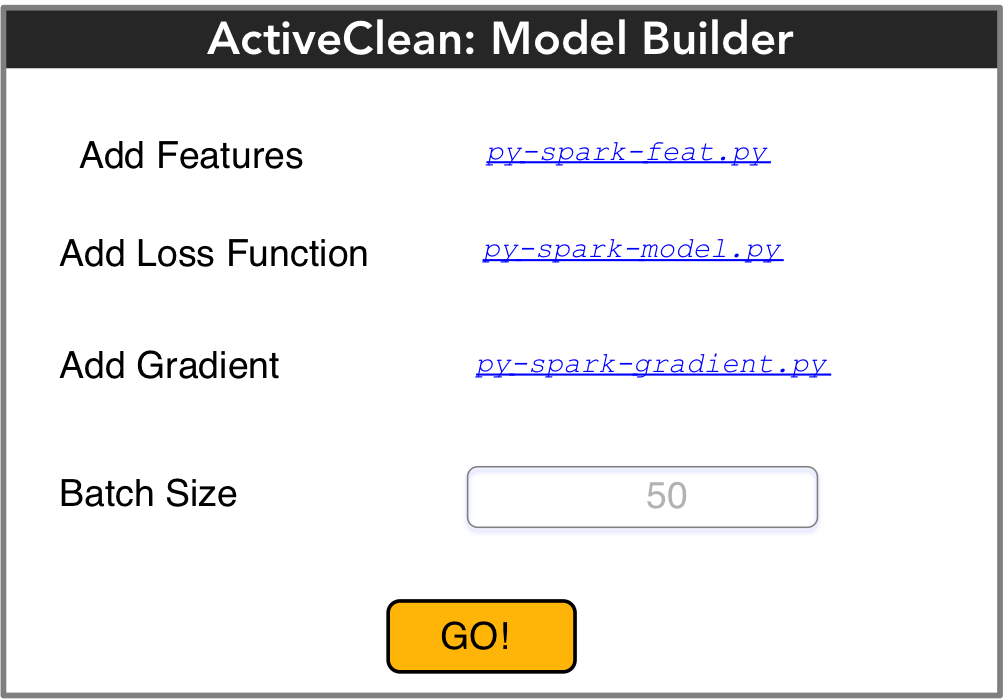
\includegraphics[width=0.48\columnwidth]{figs/interface1.png}
 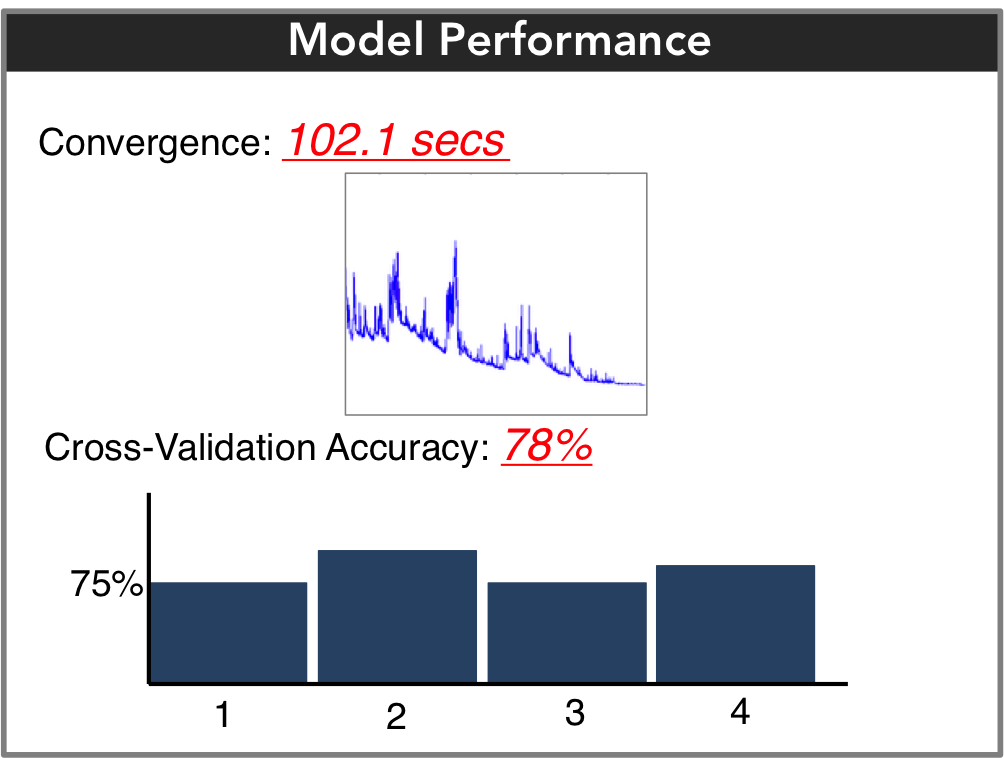
\includegraphics[width=0.48\columnwidth]{figs/interface2.png}
 \caption{Initialization. The analyst loads user-defined model functions into \sys and then trains an initial model on the dirty data \label{irun}}
\end{figure}

\subsection{Initialization}
The first part of \sys is called the \textsf{Model Builder}, this is an interface that the analyst uses to specify the problem.
She loads three user-defined functions written in PySpark~\cite{pyspark} based on the descriptions in the previous section.
Optionally, she can change the batch size from our default setting of 50.
Once the model is instantiated, then she can train the model on the dirty data.
If there are any errors that are critical, i.e., causes the training to fail, \sys will immediately error.
However, if the training proceeds to completion, the analyst will see the \textsf{Performance} window which plots the model's convergence as a function of iteration.
It also shows the cross-validation accuracy if it is a classification task and the hold-out residual error if it is a regression task.
Both of these panels are visualized in Figure \ref{irun}.

\subsection{Diagnose Interface}
Suppose the analyst is unhappy with her model, and wishes to understand why her prediction accuracy is poor.
She can then open the \textsf{Diagnose} panel to understand why (Figure \ref{diag}).
When she opens the \textsf{Diagnose} panel, \sys applies the importance sampling algorithm to select a subset of examples from the dataset.
Since these points are in general high dimensional, we apply T-SNE~\cite{van2008visualizing} to visualize the points in 2D.
The batch size setting controls the number of examples plotted on this screen.
T-SNE is a non-linear dimensionality reduction technique that is widely used to visualize complex data distributions.
In the \textsf{Diagnose} panel, we use color coding to indicate the label in the case of classification.
The analyst can select examples from the plot for further inspection.

\begin{figure}[t]
\centering
 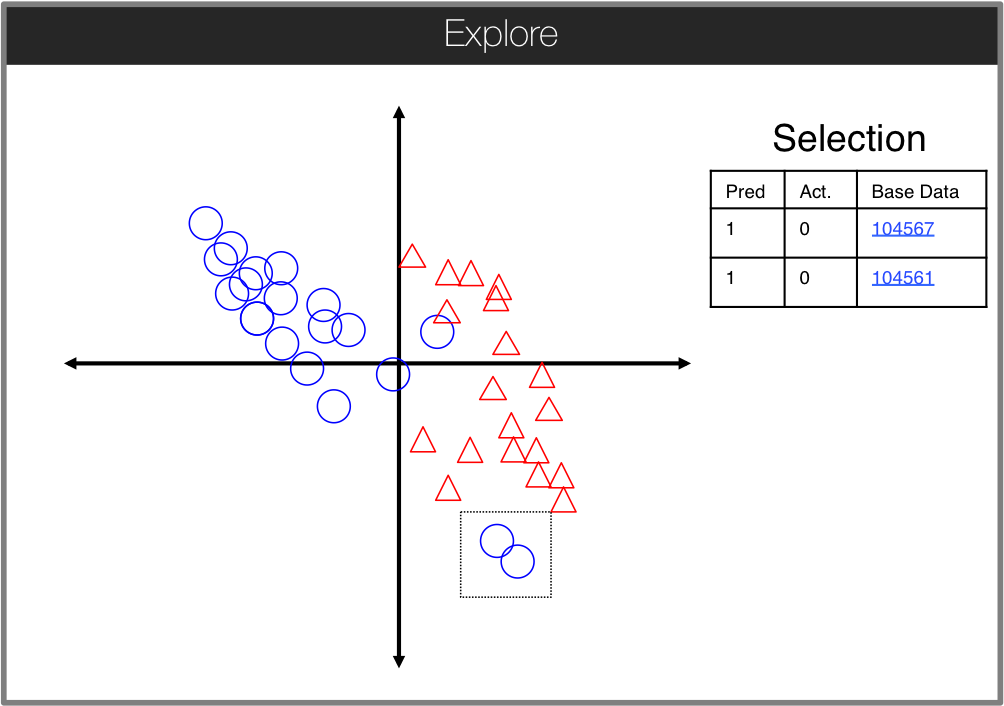
\includegraphics[width=0.6\columnwidth]{figs/interface3.png}
 \caption{The diagnose inteface. The analyst can select and inspect suspect data. \label{diag}}
\end{figure}

\subsection{Clean Interface}
If the analyst decides that the data are actually dirty, then she can open the \textsf{Clean} panel.
This panel gives her the option to remove the dirty record or apply a cleaning operation (specified in Python).
\sys keeps track of previously written cleaning operations and the analyst need not write a new script each time, and simply assign a previously written transformation. 
This serves two purposes: (1) it reduces effort for the analyst, and (2) it helps \sys taxonomize the types of errors in the dataset.
By understanding which data are similarly corrupted, we can guide future samples to draw similar data in future samples.
This may draw data not quite cleaned by the operations described in the script.
This optimization is described in detail in our technical report~\cite{activecleanarxiv}. 
Essentially, for each distinct script, \sys also trains a classifier to learn the conditions when that operation is applicable.

\begin{figure}[t]
\centering
 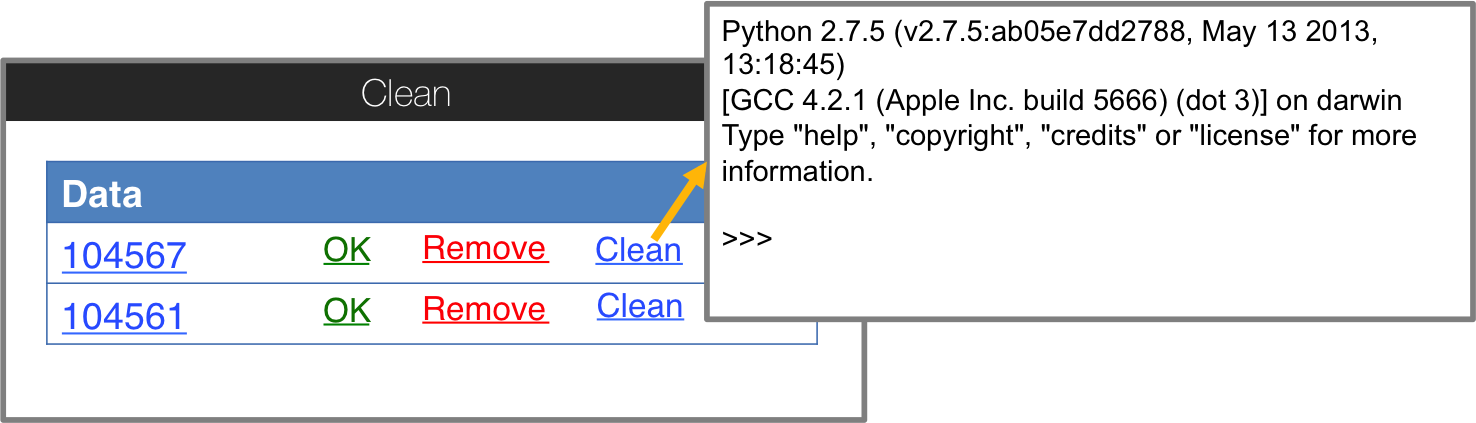
\includegraphics[width=\columnwidth]{figs/interface4.png}
 \caption{Cleaning Interface. The analyst can choose to remove data, write a custom cleaning operation, or automatically clean the data using an existing cleaning operation.}
\end{figure}

\subsection{Iteration and Updates}
Finally, after the batch of data is cleaned, \sys updates the current best model.
We re-run the cross-validation and visualize the differences in the model's accuracy (Figure~\ref{modelacc}).
This process iterates until the analyst is satisfied with the accuracy.
At that point the system ends, and returns a python pickle of current best model parameters.


\begin{figure}[t]
\centering
 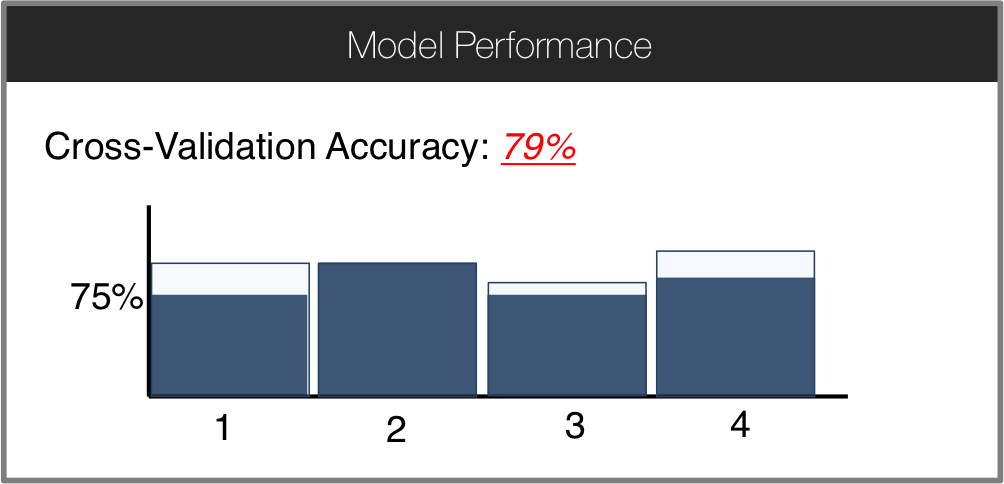
\includegraphics[width=0.6\columnwidth]{figs/interface5.png}
 \caption{Update Visualization. We visualize the changes in model accuracy after data cleaning.}\label{modelacc}
\end{figure}